
\section{Einleitung}

\subsection{Aufgabenstellung}

\begin{frame}{Einleitung}{Aufgabenstellung}
	\begin{block}{Laut Webseite \cite{web:kpgdvws14}}
		\begin{quote}
			[...] Ziel dieses Komplexpraktikums ist die indirekte Steuerung des
			Roboterarms Jaco mithilfe von Eingaben durch eine Microsoft Kinect.
		\end{quote}
	\end{block}

	\begin{block}{Im Detail}
		\begin{itemize}
			\item (Semi-)automatische Kalibrierung des Kamera-Arm-Setups
			\item Anschließende Auswahl im Kamerabild und Greifen eines Objekts
		\end{itemize}
	\end{block}
\end{frame}

\subsection{Setup}

\begin{frame}{Einleitung}{Setup}
	\begin{figure}
		\includegraphics<1>[width=0.6\textwidth]{setup_top}
		\includegraphics<2>[width=0.6\textwidth]{setup_side}
		\caption[<1>]{Kamera-Arm Setup (\only<1>{Draufsicht}\only<2>{Seitenansicht})}
	\end{figure}
\end{frame}

\subsection{Motivation}

\begin{frame}{Einleitung}{Motivation}
	\begin{block}{Aus studentischer Sicht}
		\begin{itemize}
			\item Anwendung theoretischer Kenntnisse in der Praxis
			\item Roboter sind super
		\end{itemize}
	\end{block}
	\begin{block}{Aus Lehrstuhl-Sicht}
		\begin{itemize}
			\item Fortführung der Forschung im Bereich Kalibrierung von
				Robotiksystemen
			\item Darstellung von Forschungsergebnissen in einfachem
				Anwendungsszenario
		\end{itemize}
	\end{block}
\end{frame}

\subsection{Teilaufgaben}

\begin{frame}{Einleitung}{Teilaufgaben}
	\begin{itemize}
		\item Einarbeitung
			\begin{itemize}
				\item Einrichtung der Kamera und des Arms auf den
					Zielplattformen %(Windows \& Linux)
				\item Exploration der jeweiligen Geräte-APIs
			\end{itemize}
		\item Schnittstellenspezifikation und -implementierung
		\item Erkennung und Kalibrierung
			\begin{itemize}
				\item Positionierung des Arms an verschiedenen Punkten
				\item Erkennung der Endeffektorposition im Kinect-Bild
				\item Starrkörpertransformation
			\end{itemize}
		\item Anfahren und Greifen des Objektes durch den Arm
	\end{itemize}
\end{frame}

\subsection{Architektur}

\begin{frame}[b]{Einleitung}{Softwarekomponenten}
	\begin{figure}
		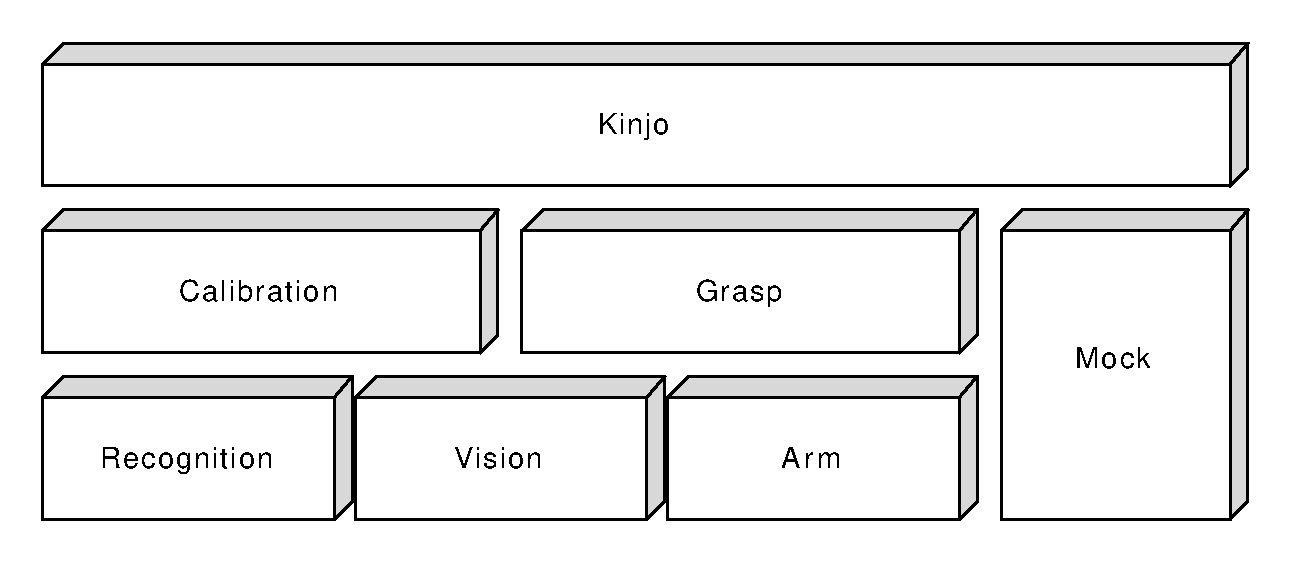
\includegraphics[width=0.8\textwidth]{architecture}
	\end{figure}
	\vspace*{0.7cm}
\end{frame}

